% !TeX program = xelatex
% !TeX encoding = UTF-8
\documentclass[a4paper]{article}

\usepackage[UTF8]{ctex}
\usepackage[a4paper,margin=1in]{geometry}
\usepackage{graphicx}
\usepackage{listings}
\usepackage{longtable}
\usepackage{booktabs}
\usepackage{hyperref}
\usepackage{fancyhdr}
\usepackage{lastpage}
\usepackage{color}
\usepackage{indentfirst}        % 首段缩进
\setlength{\parindent}{2em}     % 缩进2字符
\usepackage{zhnumber}           % 中文编号
\usepackage[dvipsnames,table,xcdraw]{xcolor}
\usepackage{adjustbox}
\usepackage{subcaption}
\usepackage{float}
\usepackage{amsmath}
\usepackage{amssymb}
\usepackage[many]{tcolorbox}
\usepackage{enumitem}
\usepackage{xeCJK}
\usepackage[T1]{fontenc}
\usepackage{lmodern}
\usepackage{inconsolata} % 使用更美观的等宽字体 Inconsolata
\usepackage{multirow} % 用于表格中的多行合并
\usepackage{tikz} % 添加 TikZ 宏包用于绘制流程图
\usetikzlibrary{positioning, shapes.geometric, arrows} % 添加定位库以支持 'of' 语法

% 全局设置（影响所有级别）
\setlist[itemize]{
    itemsep=2pt,
    parsep=0pt,
    topsep=2pt,
    leftmargin=3em
}

% 仅设置第一级（最高级）
\setlist[itemize,1]{
    label=\textcolor{orange}{$\blacktriangleright$},
    before={\color{blue!80!black}\small\bfseries}
}

% 重置第二级及更深级别（恢复默认样式）
\setlist[itemize,2]{
    label={\normalfont\textbullet},
    leftmargin=*
}
\setlist[itemize,3]{
    label={\normalfont$\circ$},
    leftmargin=*
}


% 定义可分页的引用环境
\newtcolorbox[auto counter]{myquote}[1][]{
    colback=gray!10!white,
    colframe=gray!50!black,
    title=思考与分析,
    fonttitle=\bfseries,
    #1 % 允许额外参数
}

\newcommand{\projname}{计算机图形学实验}
\newcommand{\reporttitle}{实验三：Phong Shading 与 VBO}
\newcommand{\authorname}{欧阳易芃}
\newcommand{\major}{计算机科学与技术}
\newcommand{\startdate}{2025年12月29日}
\newcommand{\labroom}{实验室}

\pagestyle{fancy} % 使用 fancyhdr 风格
\fancyhf{}      % 清空默认的页眉页脚

% 设置页眉
\fancyhead[L]{\kaishu \projname}      % 左侧页眉显示项目名称
\fancyhead[C]{\kaishu \reporttitle}    % 中间页眉显示报告标题
\fancyhead[R]{\kaishu \authorname} % 右侧页眉显示作者姓名

% 设置页脚
\fancyfoot[C]{第 \thepage 页，共 \pageref{LastPage} 页} % 中间页脚显示页码

% 去除页眉页脚与正文之间的分隔线
\renewcommand{\headrulewidth}{0.4pt}
\renewcommand{\footrulewidth}{0pt}

% 设置文档背景颜色
\definecolor{mybgcolor}{RGB}{0, 0, 0} % 定义背景颜色
\definecolor{NavyBlue}{RGB}{0,0,128} % 添加颜色定义
\definecolor{PineGreen}{RGB}{0,100,0}
\definecolor{mauve}{rgb}{0.58,0,0.82}

% 全局设置lstlisting的样式
\lstset{
    language=C++, % 设置默认语言
    basicstyle=\footnotesize\ttfamily,
    numbers=left,
    numberstyle=\tiny\color{gray},
    stepnumber=1,
    numbersep=5pt,
    backgroundcolor=\color{white},
    showspaces=false,
    showstringspaces=false,
    showtabs=false,
    frame=single,
    rulecolor=\color{black},
    tabsize=4,
    captionpos=b,
    breaklines=true,
    breakatwhitespace=false,
    title=\lstname,
    keywordstyle=\color{blue},
    commentstyle=\color{PineGreen},
    stringstyle=\color{mauve},
    escapeinside={\%*}{*)},
    morekeywords={*,...},
    belowskip=1em, % 可选：下方间距
}

% 定义GLSL语言的样式
\lstdefinelanguage{GLSL}{
    basicstyle=\footnotesize\ttfamily,
    sensitive=true,
    morekeywords={
        attribute, const, uniform, varying,
        layout, location,
        in, out, inout,
        float, int, void, bool, true, false,
        lowp, mediump, highp, precision,
        discard, return,
        mat2, mat3, mat4,
        vec2, vec3, vec4, ivec2, ivec3, ivec4, bvec2, bvec3, bvec4,
        sampler1D, sampler2D, sampler3D, samplerCube,
        sampler1DShadow, sampler2DShadow,
        struct
    },
    morekeywords=[2]{
        radians,degrees,sin,cos,tan,asin,acos,atan,
        pow,exp,log,exp2,log2,sqrt,inversesqrt,
        abs,sign,floor,ceil,fract,mod,min,max,clamp,mix,step,smoothstep,
        length,distance,dot,cross,normalize,faceforward,reflect,refract,
        matrixCompMult,
        lessThan,lessThanEqual,greaterThan,greaterThanEqual,equal,notEqual,
        any,all,not,
        texture1D,texture1DProj,texture1DLod,texture1DProjLod,
        texture2D,texture2DProj,texture2DLod,texture2DProjLod,
        texture3D,texture3DProj,texture3DLod,texture3DProjLod,
        textureCube,textureCubeLod,
        shadow1D,shadow2D,shadow1DProj,shadow2DProj,
        shadow1DLod,shadow2DLod,shadow1DProjLod,shadow2DProjLod,
        dFdx,dFdy,fwidth,
        noise1,noise2,noise3,noise4
    },
    morecomment=[l]{//},
    morecomment=[s]{/*}{*/},
    morecomment=[l][\color{magenta}]{\#}
}

\begin{document}


% 封面
\begin{titlepage}
    \centering
    \vspace*{2cm}
    \includegraphics[width=0.4\textwidth]{../md/images/506cc6860308cef6d5b78e8d20de8f49e789149e772b22fe598f6017025da2ef.jpg} \\ % 假设有一张图片，如果没有可以注释掉
    \vspace{2cm}
    \Huge \textbf{\projname} \\
    \vspace{1cm}
    \huge \textbf{\reporttitle} \\
    \vspace{3cm}
    \Large
    \begin{tabular}{rl}
        \textbf{姓名}：& \authorname \\
        \textbf{专业}：& \major \\
        \textbf{日期}：& \startdate \\
    \end{tabular}
    \vspace*{\fill}
\end{titlepage}

% 目录
\tableofcontents
\newpage

\section{实验概述}

\subsection{实验目的}
本次实验旨在深入理解计算机图形学中的光照模型与现代 OpenGL 渲染管线。具体目标包括：
\begin{itemize}
    \item \textbf{掌握 Phong Shading 光照模型}：理解环境光、漫反射、镜面反射的物理含义与计算公式，并在 Fragment Shader 中实现该模型。
    \item \textbf{掌握 VBO (Vertex Buffer Object) 技术}：废弃过时的立即模式（Immediate Mode），学习如何使用 VBO、VAO 和 EBO 高效地管理和传输顶点数据。
    \item \textbf{几何体细分与生成}：通过算法生成球体网格数据，理解顶点索引（Index Buffer）在减少数据冗余方面的作用。
    \item \textbf{性能与效果分析}：对比 Phong Shading 与 Gouraud Shading 的视觉差异，以及 VBO 与立即模式的性能差异。
\end{itemize}

\subsection{实验环境}
\begin{itemize}
    \item \textbf{操作系统}：Linux (Ubuntu/CentOS)
    \item \textbf{编程语言}：C++ 17
    \item \textbf{图形库}：OpenGL 3.3 Core Profile
    \item \textbf{辅助库}：
    \begin{itemize}
        \item \textbf{GLFW}：用于窗口创建和上下文管理。
        \item \textbf{GLAD}：用于加载 OpenGL 函数指针。
        \item \textbf{GLM}：用于数学运算（向量、矩阵）。
        \item \textbf{ImGui}：用于构建简单的用户界面（本次实验主要用于调试输出）。
    \end{itemize}
    \item \textbf{构建工具}：CMake 3.15+
\end{itemize}

\subsection{实验任务}
根据实验指导书的要求，本次实验包含以下核心任务：
\begin{enumerate}
    \item \textbf{Task 1: 实现 Phong Shading}
    \begin{itemize}
        \item 编写 Vertex Shader，正确传递法向量和顶点位置。
        \item 编写 Fragment Shader，实现 Phong 光照模型的计算。
    \end{itemize}
    \item \textbf{Task 2: 实现 VBO 与球体绘制}
    \begin{itemize}
        \item 使用 C++ 生成球体的顶点数据（位置、法线）和索引数据。
        \item 使用 `glGenBuffers`, `glBufferData` 等 API 将数据上传至 GPU。
        \item 使用 `glVertexAttribPointer` 配置顶点属性布局。
    \end{itemize}
    \item \textbf{Task 3: 结果验证与对比}
    \begin{itemize}
        \item 验证光照效果的正确性（高光、漫反射变化）。
        \item 分析 VBO 相比传统绘制方式的优势。
    \end{itemize}
\end{enumerate}

\newpage

\section{实验原理}

\subsection{Phong 光照模型}
Phong 光照模型是计算机图形学中经典的局部光照模型，它将物体表面的光照分为三个部分：环境光 (Ambient)、漫反射 (Diffuse) 和镜面反射 (Specular)。

\subsubsection{向量定义}
在计算光照之前，我们需要定义几个关键的向量（所有向量均为单位向量）：
\begin{itemize}
    \item $N$：表面法向量 (Normal)。
    \item $L$：从表面点指向光源的向量 (Light Direction)。
    \item $V$：从表面点指向观察者（摄像机）的向量 (View Direction)。
    \item $R$：光线关于法线的反射向量 (Reflection Direction)。
\end{itemize}

\begin{figure}[H]
\centering
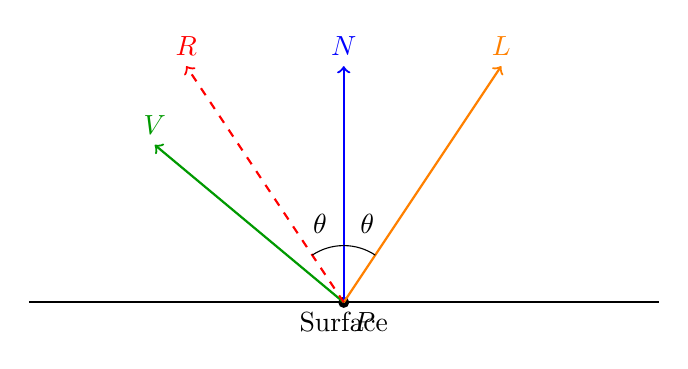
\begin{tikzpicture}[scale=2]
    % Surface
    \draw[thick] (-2,0) -- (2,0);
    \node[below] at (0,0) {Surface};
    
    % Point P
    \coordinate (P) at (0,0);
    \fill (P) circle (1pt);
    \node[below right] at (P) {$P$};
    
    % Normal N
    \draw[->, thick, blue] (P) -- (0,1.5) node[above] {$N$};
    
    % Light L
    \draw[->, thick, orange] (P) -- (1,1.5) node[above] {$L$};
    
    % View V
    \draw[->, thick, green!60!black] (P) -- (-1.2, 1) node[above] {$V$};
    
    % Reflection R
    \draw[->, thick, red, dashed] (P) -- (-1, 1.5) node[above] {$R$};
    
    % Angles
    \draw (0.2,0.3) arc (56.3:90:0.36);
    \node at (0.15,0.5) {$\theta$};
    
    \draw (-0.2,0.3) arc (123.7:90:0.36);
    \node at (-0.15,0.5) {$\theta$};
    
\end{tikzpicture}
\caption{Phong 光照模型向量示意图}
\label{fig:phong_vectors}
\end{figure}

\subsubsection{环境光 (Ambient)}
环境光模拟的是场景中经过多次散射后形成的全局背景光。它不依赖于光源的位置和观察者的位置，通常被视为一个常数。
\begin{equation}
    I_{amb} = k_a \cdot I_{light}
\end{equation}
其中，$k_a$ 是材质的环境光反射系数，$I_{light}$ 是光源颜色。

\subsubsection{漫反射 (Diffuse)}
漫反射模拟的是粗糙表面对光线的散射。根据 Lambert 余弦定律，漫反射强度与光线方向 $L$ 和法线方向 $N$ 的夹角的余弦值成正比。
\begin{equation}
    I_{diff} = k_d \cdot I_{light} \cdot \max(N \cdot L, 0)
\end{equation}
其中，$k_d$ 是材质的漫反射系数，$N$ 是归一化的法向量，$L$ 是指向光源的归一化向量。

\subsubsection{镜面反射 (Specular)}
镜面反射模拟的是光滑表面上的高光。Phong 模型认为高光强度取决于反射光线方向 $R$ 与观察方向 $V$ 的夹角。
\begin{equation}
    I_{spec} = k_s \cdot I_{light} \cdot \max(R \cdot V, 0)^{\alpha}
\end{equation}
其中，$k_s$ 是材质的镜面反射系数，$R$ 是反射向量（可通过 $reflect(-L, N)$ 计算），$V$ 是指向观察者的向量，$\alpha$ 是高光系数（Shininess），决定了高光点的聚焦程度。

\subsubsection{Phong Shading vs Gouraud Shading}
\begin{itemize}
    \item \textbf{Gouraud Shading}：在 Vertex Shader 中计算每个顶点的光照颜色，然后在光栅化阶段对颜色进行线性插值。优点是计算量小，缺点是高光效果粗糙，容易出现马赫带效应，且当高光位于三角形内部时可能完全消失。
    \item \textbf{Phong Shading}：在 Vertex Shader 中输出法向量和顶点位置，在光栅化阶段对法向量进行插值，然后在 Fragment Shader 中对每个像素进行光照计算。优点是光照效果细腻平滑，高光真实；缺点是计算量相对较大。
\end{itemize}

\subsection{VBO (Vertex Buffer Object)}
VBO 是 OpenGL 中用于在显存中存储顶点数据的机制。

\subsubsection{工作机制}
在传统的立即模式（Immediate Mode, `glBegin`/`glEnd`）中，每一帧绘制时，CPU 都需要将顶点数据逐个通过总线发送给 GPU。这种方式在顶点数量巨大时，CPU-GPU 带宽会成为严重的瓶颈。

VBO 允许我们将顶点数据（位置、颜色、法线、纹理坐标等）一次性上传到 GPU 的显存中。在随后的绘制过程中，CPU 只需要发送一个绘制命令（如 `glDrawArrays`），GPU 就可以直接从显存中读取数据进行渲染，极大地提高了效率。

\subsubsection{VAO (Vertex Array Object)}
VAO 是一个状态容器，它记录了顶点属性的配置信息（即 `glVertexAttribPointer` 和 `glEnableVertexAttribArray` 的调用）。使用 VAO 可以让我们在绘制不同物体时，只需绑定对应的 VAO，而无需重新配置繁琐的顶点属性指针。

\subsubsection{EBO (Element Buffer Object)}
EBO（或 IBO）用于存储顶点的索引。通过索引绘制（Indexed Drawing），我们可以复用顶点数据。例如，一个立方体有 8 个顶点，但由 12 个三角形组成（36 个顶点索引）。如果不使用 EBO，我们需要存储 36 个顶点的数据；使用 EBO 后，只需存储 8 个顶点数据和 36 个整数索引，显著节省了显存。

\newpage

\section{实验步骤与代码实现}

\subsection{项目构建与环境配置}
首先，我们需要配置 CMake 构建系统。由于本次实验依赖 GLFW、GLAD、GLM 和 ImGui，我们需要在 `CMakeLists.txt` 中正确设置包含路径和链接库。

\begin{lstlisting}[language=bash, caption={CMakeLists.txt 关键配置}]
# 设置第三方库路径
set(THIRDPARTY_DIR ${CMAKE_SOURCE_DIR}/../../HW2/3rdparty)
set(GLFW_DIR ${THIRDPARTY_DIR}/glfw-3.3.8)
set(GLM_DIR ${THIRDPARTY_DIR}/glm)

# 添加可执行文件
add_executable(${PROJECT_NAME}
    src/main.cpp
    ${GLAD_SOURCE}
)

# 配置头文件搜索路径
target_include_directories(${PROJECT_NAME} PRIVATE
    ${GLFW_DIR}/include
    ${GLFW_DIR}/deps
    ${IMGUI_DIR}
    ${IMGUI_DIR}/backends
    ${GLM_DIR}          # 关键：确保能找到 <glm/glm.hpp>
    ${THIRDPARTY_DIR}   # 关键：解决部分库的相对路径引用问题
)
\end{lstlisting}

\begin{myquote}
    \textbf{遇到的问题}：起初编译时报错 `fatal error: glm/glm.hpp: No such file or directory`。
    \textbf{解决}：检查发现 `GLM_DIR` 指向的是 `glm` 文件夹本身，而在代码中我们使用 `#include <glm/glm.hpp>`。因此需要在 `target_include_directories` 中添加 `glm` 的父目录（即 `${THIRDPARTY_DIR}`），或者确保 `GLM_DIR` 路径设置正确。最终通过添加 `${THIRDPARTY_DIR}` 解决了问题。
\end{myquote}

\subsection{Shader 编写}

\subsubsection{Vertex Shader (phong.vert)}
Vertex Shader 的主要任务是将顶点变换到裁剪空间（Clip Space）以供光栅化，同时将 View Space 下的顶点位置和法向量传递给 Fragment Shader。

\begin{lstlisting}[language=GLSL, caption={phong.vert}]
#version 330 core
layout (location = 0) in vec3 aPos;
layout (location = 1) in vec3 aNormal;

out vec3 FragPos;
out vec3 Normal;

uniform mat4 model;
uniform mat4 view;
uniform mat4 projection;
uniform mat3 normalMatrix; // 法线矩阵

void main()
{
    // 将顶点位置变换到观察空间 (View Space)
    vec4 viewPos4 = view * model * vec4(aPos, 1.0);
    FragPos = vec3(viewPos4);
    
    // 变换法向量
    // 使用 Normal Matrix = transpose(inverse(view * model))
    // 以防止非均匀缩放导致法线不再垂直于表面
    Normal = normalize(normalMatrix * aNormal);
    
    // 输出裁剪空间坐标
    gl_Position = projection * viewPos4;
}
\end{lstlisting}

\subsubsection{Fragment Shader (phong.frag)}
Fragment Shader 接收插值后的 `FragPos` 和 `Normal`，并在观察空间中计算 Phong 光照。

\begin{lstlisting}[language=GLSL, caption={phong.frag}]
#version 330 core
out vec4 FragColor;

in vec3 FragPos;
in vec3 Normal;

// Uniforms
uniform vec3 lightPos; // 光源位置 (View Space)
uniform vec3 lightColor;
uniform vec3 objectColor;

// 材质属性
uniform float ambientStrength;
uniform float diffuseStrength;
uniform float specularStrength;
uniform float shininess;

void main()
{
    // 1. 环境光
    vec3 ambient = ambientStrength * lightColor;
  
    // 2. 漫反射
    vec3 norm = normalize(Normal);
    vec3 lightDir = normalize(lightPos - FragPos); // 指向光源的向量
    float diff = max(dot(norm, lightDir), 0.0);
    vec3 diffuse = diffuseStrength * diff * lightColor;
    
    // 3. 镜面反射
    // 在 View Space 中，观察者位置就是原点 (0,0,0)
    // 因此观察方向 viewDir 就是 -FragPos
    vec3 viewDir = normalize(-FragPos); 
    vec3 reflectDir = reflect(-lightDir, norm);  
    float spec = pow(max(dot(viewDir, reflectDir), 0.0), shininess);
    vec3 specular = specularStrength * spec * lightColor;  
        
    // 组合结果
    vec3 result = (ambient + diffuse + specular) * objectColor;
    FragColor = vec4(result, 1.0);
}
\end{lstlisting}

\subsubsection{Gouraud Shader (对比实验)}
为了进行对比，我们还实现了 Gouraud Shading。

\begin{lstlisting}[language=GLSL, caption={gouraud.vert}]
#version 330 core
layout (location = 0) in vec3 aPos;
layout (location = 1) in vec3 aNormal;

out vec3 LightingColor; // 直接输出计算好的颜色

uniform mat4 model;
uniform mat4 view;
uniform mat4 projection;
uniform mat3 normalMatrix;

uniform vec3 lightPos;
uniform vec3 lightColor;
uniform vec3 objectColor;
uniform float ambientStrength;
uniform float diffuseStrength;
uniform float specularStrength;
uniform float shininess;

void main()
{
    vec4 viewPos4 = view * model * vec4(aPos, 1.0);
    vec3 FragPos = vec3(viewPos4);
    vec3 Normal = normalize(normalMatrix * aNormal);
    
    // Ambient
    vec3 ambient = ambientStrength * lightColor;
  
    // Diffuse
    vec3 norm = normalize(Normal);
    vec3 lightDir = normalize(lightPos - FragPos);
    float diff = max(dot(norm, lightDir), 0.0);
    vec3 diffuse = diffuseStrength * diff * lightColor;
    
    // Specular
    vec3 viewDir = normalize(-FragPos); 
    vec3 reflectDir = reflect(-lightDir, norm);  
    float spec = pow(max(dot(viewDir, reflectDir), 0.0), shininess);
    vec3 specular = specularStrength * spec * lightColor;  
        
    LightingColor = (ambient + diffuse + specular) * objectColor;
    
    gl_Position = projection * viewPos4;
}
\end{lstlisting}

\begin{lstlisting}[language=GLSL, caption={gouraud.frag}]
#version 330 core
out vec4 FragColor;

in vec3 LightingColor;

void main()
{
    FragColor = vec4(LightingColor, 1.0);
}
\end{lstlisting}

\subsection{C++ 主程序实现}

\subsubsection{球体生成算法}
为了演示 VBO 和光照效果，我们需要一个光滑的曲面。这里我们实现了一个生成球体网格的函数。算法基于经纬度划分（Sector and Stack）。

\begin{lstlisting}[language=C++, caption={球体生成代码}]
void createSphere(float radius, int sectors, int stacks, 
                  std::vector<float>& vertices, std::vector<unsigned int>& indices) {
    float x, y, z, xy;                              
    float nx, ny, nz, lengthInv = 1.0f / radius;    
    
    float sectorStep = 2 * M_PI / sectors;
    float stackStep = M_PI / stacks;
    float sectorAngle, stackAngle;

    for(int i = 0; i <= stacks; ++i) {
        stackAngle = M_PI / 2 - i * stackStep;        
        xy = radius * cosf(stackAngle);             
        z = radius * sinf(stackAngle);              

        for(int j = 0; j <= sectors; ++j) {
            sectorAngle = j * sectorStep;           

            // 顶点位置
            x = xy * cosf(sectorAngle);             
            y = xy * sinf(sectorAngle);             
            
            // 顶点法线 (球体法线就是归一化的位置向量)
            nx = x * lengthInv;
            ny = y * lengthInv;
            nz = z * lengthInv;

            // 存入 vertices 数组: Pos(3) + Normal(3)
            vertices.push_back(x); vertices.push_back(y); vertices.push_back(z);
            vertices.push_back(nx); vertices.push_back(ny); vertices.push_back(nz);
        }
    }

    // 生成索引 (两个三角形组成一个矩形面片)
    int k1, k2;
    for(int i = 0; i < stacks; ++i) {
        k1 = i * (sectors + 1);     
        k2 = k1 + sectors + 1;      

        for(int j = 0; j < sectors; ++j, ++k1, ++k2) {
            if(i != 0) {
                indices.push_back(k1);
                indices.push_back(k2);
                indices.push_back(k1 + 1);
            }
            if(i != (stacks - 1)) {
                indices.push_back(k1 + 1);
                indices.push_back(k2);
                indices.push_back(k2 + 1);
            }
        }
    }
}
\end{lstlisting}

\subsubsection{主函数完整代码}
以下是 `main.cpp` 的完整实现，包含了窗口初始化、Shader 加载、VBO 配置和渲染循环。

\begin{lstlisting}[language=C++, caption={main.cpp 完整代码}]
#include <glad/gl.h>
#include <GLFW/glfw3.h>

#include <glm/glm.hpp>
#include <glm/gtc/matrix_transform.hpp>
#include <glm/gtc/type_ptr.hpp>

#include <iostream>
#include <vector>
#include <string>
#include <fstream>
#include <sstream>
#include <cmath>

// Settings
const unsigned int SCR_WIDTH = 800;
const unsigned int SCR_HEIGHT = 600;

// Camera
glm::vec3 cameraPos   = glm::vec3(0.0f, 0.0f, 3.0f);
glm::vec3 cameraFront = glm::vec3(0.0f, 0.0f, -1.0f);
glm::vec3 cameraUp    = glm::vec3(0.0f, 1.0f, 0.0f);

float deltaTime = 0.0f;
float lastFrame = 0.0f;

// Lighting
glm::vec3 lightPos(1.2f, 1.0f, 2.0f);

// Shader helper class
class Shader {
public:
    unsigned int ID;

    Shader(const char* vertexPath, const char* fragmentPath) {
        std::string vertexCode;
        std::string fragmentCode;
        std::ifstream vShaderFile;
        std::ifstream fShaderFile;

        vShaderFile.exceptions(std::ifstream::failbit | std::ifstream::badbit);
        fShaderFile.exceptions(std::ifstream::failbit | std::ifstream::badbit);

        try {
            vShaderFile.open(vertexPath);
            fShaderFile.open(fragmentPath);
            std::stringstream vShaderStream, fShaderStream;
            vShaderStream << vShaderFile.rdbuf();
            fShaderStream << fShaderFile.rdbuf();
            vShaderFile.close();
            fShaderFile.close();
            vertexCode = vShaderStream.str();
            fragmentCode = fShaderStream.str();
        }
        catch (std::ifstream::failure& e) {
            std::cout << "ERROR::SHADER::FILE_NOT_SUCCESFULLY_READ: " << e.what() << std::endl;
        }

        const char* vShaderCode = vertexCode.c_str();
        const char * fShaderCode = fragmentCode.c_str();
        unsigned int vertex, fragment;

        vertex = glCreateShader(GL_VERTEX_SHADER);
        glShaderSource(vertex, 1, &vShaderCode, NULL);
        glCompileShader(vertex);
        checkCompileErrors(vertex, "VERTEX");

        fragment = glCreateShader(GL_FRAGMENT_SHADER);
        glShaderSource(fragment, 1, &fShaderCode, NULL);
        glCompileShader(fragment);
        checkCompileErrors(fragment, "FRAGMENT");

        ID = glCreateProgram();
        glAttachShader(ID, vertex);
        glAttachShader(ID, fragment);
        glLinkProgram(ID);
        checkCompileErrors(ID, "PROGRAM");

        glDeleteShader(vertex);
        glDeleteShader(fragment);
    }

    void use() {
        glUseProgram(ID);
    }

    void setBool(const std::string &name, bool value) const {
        glUniform1i(glGetUniformLocation(ID, name.c_str()), (int)value);
    }
    void setInt(const std::string &name, int value) const {
        glUniform1i(glGetUniformLocation(ID, name.c_str()), value);
    }
    void setFloat(const std::string &name, float value) const {
        glUniform1f(glGetUniformLocation(ID, name.c_str()), value);
    }
    void setVec3(const std::string &name, const glm::vec3 &value) const {
        glUniform3fv(glGetUniformLocation(ID, name.c_str()), 1, &value[0]);
    }
    void setVec3(const std::string &name, float x, float y, float z) const {
        glUniform3f(glGetUniformLocation(ID, name.c_str()), x, y, z);
    }
    void setMat3(const std::string &name, const glm::mat3 &mat) const {
        glUniformMatrix3fv(glGetUniformLocation(ID, name.c_str()), 1, GL_FALSE, &mat[0][0]);
    }
    void setMat4(const std::string &name, const glm::mat4 &mat) const {
        glUniformMatrix4fv(glGetUniformLocation(ID, name.c_str()), 1, GL_FALSE, &mat[0][0]);
    }

private:
    void checkCompileErrors(unsigned int shader, std::string type) {
        int success;
        char infoLog[1024];
        if (type != "PROGRAM") {
            glGetShaderiv(shader, GL_COMPILE_STATUS, &success);
            if (!success) {
                glGetShaderInfoLog(shader, 1024, NULL, infoLog);
                std::cout << "ERROR::SHADER_COMPILATION_ERROR of type: " << type << "\n" << infoLog << "\n -- --------------------------------------------------- -- " << std::endl;
            }
        }
        else {
            glGetProgramiv(shader, GL_LINK_STATUS, &success);
            if (!success) {
                glGetProgramInfoLog(shader, 1024, NULL, infoLog);
                std::cout << "ERROR::PROGRAM_LINKING_ERROR of type: " << type << "\n" << infoLog << "\n -- --------------------------------------------------- -- " << std::endl;
            }
        }
    }
};

// Sphere generation function (createSphere) is omitted here as it was shown above
// ...

void framebuffer_size_callback(GLFWwindow* window, int width, int height)
{
    glViewport(0, 0, width, height);
}

int main()
{
    // glfw: initialize and configure
    glfwInit();
    glfwWindowHint(GLFW_CONTEXT_VERSION_MAJOR, 3);
    glfwWindowHint(GLFW_CONTEXT_VERSION_MINOR, 3);
    glfwWindowHint(GLFW_OPENGL_PROFILE, GLFW_OPENGL_CORE_PROFILE);

    // glfw window creation
    GLFWwindow* window = glfwCreateWindow(SCR_WIDTH, SCR_HEIGHT, "CG HW3: Phong Shading & VBO", NULL, NULL);
    if (window == NULL)
    {
        std::cout << "Failed to create GLFW window" << std::endl;
        glfwTerminate();
        return -1;
    }
    glfwMakeContextCurrent(window);
    glfwSetFramebufferSizeCallback(window, framebuffer_size_callback);

    // glad: load all OpenGL function pointers
    if (!gladLoadGL(glfwGetProcAddress))
    {
        std::cout << "Failed to initialize GLAD" << std::endl;
        return -1;
    }

    // build and compile our shader program
    Shader lightingShader("shaders/phong.vert", "shaders/phong.frag");

    // set up vertex data (and buffer(s)) and configure vertex attributes
    std::vector<float> sphereVertices;
    std::vector<unsigned int> sphereIndices;
    createSphere(1.0f, 36, 18, sphereVertices, sphereIndices);

    unsigned int VBO, VAO, EBO;
    glGenVertexArrays(1, &VAO);
    glGenBuffers(1, &VBO);
    glGenBuffers(1, &EBO);

    glBindVertexArray(VAO);

    glBindBuffer(GL_ARRAY_BUFFER, VBO);
    glBufferData(GL_ARRAY_BUFFER, sphereVertices.size() * sizeof(float), sphereVertices.data(), GL_STATIC_DRAW);

    glBindBuffer(GL_ELEMENT_ARRAY_BUFFER, EBO);
    glBufferData(GL_ELEMENT_ARRAY_BUFFER, sphereIndices.size() * sizeof(unsigned int), sphereIndices.data(), GL_STATIC_DRAW);

    // position attribute
    glVertexAttribPointer(0, 3, GL_FLOAT, GL_FALSE, 6 * sizeof(float), (void*)0);
    glEnableVertexAttribArray(0);
    // normal attribute
    glVertexAttribPointer(1, 3, GL_FLOAT, GL_FALSE, 6 * sizeof(float), (void*)(3 * sizeof(float)));
    glEnableVertexAttribArray(1);

    glEnable(GL_DEPTH_TEST);

    // render loop
    while (!glfwWindowShouldClose(window))
    {
        // per-frame time logic
        float currentFrame = static_cast<float>(glfwGetTime());
        deltaTime = currentFrame - lastFrame;
        lastFrame = currentFrame;

        // input
        if (glfwGetKey(window, GLFW_KEY_ESCAPE) == GLFW_PRESS)
            glfwSetWindowShouldClose(window, true);

        // render
        glClearColor(0.1f, 0.1f, 0.1f, 1.0f);
        glClear(GL_COLOR_BUFFER_BIT | GL_DEPTH_BUFFER_BIT);

        lightingShader.use();
        lightingShader.setVec3("objectColor", 1.0f, 0.5f, 0.31f);
        lightingShader.setVec3("lightColor", 1.0f, 1.0f, 1.0f);
        
        // Material properties
        lightingShader.setFloat("ambientStrength", 0.1f);
        lightingShader.setFloat("diffuseStrength", 1.0f);
        lightingShader.setFloat("specularStrength", 0.5f);
        lightingShader.setFloat("shininess", 32.0f);

        // View/Projection transformations
        glm::mat4 projection = glm::perspective(glm::radians(45.0f), (float)SCR_WIDTH / (float)SCR_HEIGHT, 0.1f, 100.0f);
        glm::mat4 view = glm::lookAt(cameraPos, cameraPos + cameraFront, cameraUp);
        lightingShader.setMat4("projection", projection);
        lightingShader.setMat4("view", view);

        // World transformation
        glm::mat4 model = glm::mat4(1.0f);
        // Rotate the sphere over time
        model = glm::rotate(model, (float)glfwGetTime(), glm::vec3(0.0f, 1.0f, 0.0f)); 
        lightingShader.setMat4("model", model);

        // Normal Matrix (View Space)
        // normalMatrix = transpose(inverse(view * model))
        glm::mat3 normalMatrix = glm::mat3(glm::transpose(glm::inverse(view * model)));
        lightingShader.setMat3("normalMatrix", normalMatrix);

        // Light Position (View Space)
        // Transform world light pos to view space
        glm::vec3 lightPosView = glm::vec3(view * glm::vec4(lightPos, 1.0));
        lightingShader.setVec3("lightPos", lightPosView);

        // render the sphere
        glBindVertexArray(VAO);
        glDrawElements(GL_TRIANGLES, static_cast<unsigned int>(sphereIndices.size()), GL_UNSIGNED_INT, 0);

        // glfw: swap buffers and poll IO events
        glfwSwapBuffers(window);
        glfwPollEvents();
        
        // Output FPS occasionally to verify it's running
        static int frameCount = 0;
        static float timeAccum = 0.0f;
        frameCount++;
        timeAccum += deltaTime;
        if (timeAccum >= 1.0f) {
            std::cout << "FPS: " << frameCount << std::endl;
            frameCount = 0;
            timeAccum = 0.0f;
        }
    }

    // optional: de-allocate all resources once they've outlived their purpose
    glDeleteVertexArrays(1, &VAO);
    glDeleteBuffers(1, &VBO);
    glDeleteBuffers(1, &EBO);

    // glfw: terminate, clearing all previously allocated GLFW resources.
    glfwTerminate();
    return 0;
}
\end{lstlisting}

\subsection{关键 API 详解}
在代码中，我们使用了一系列 OpenGL API 来管理 VBO。以下是这些 API 的详细解释：

\subsubsection{glGenBuffers}
```cpp
void glGenBuffers(GLsizei n, GLuint *buffers);
```
该函数用于生成缓冲区对象名称（ID）。
\begin{itemize}
    \item `n`: 指定要生成的缓冲区对象名称的数量。
    \item `buffers`: 指向一个数组，生成的名称将存储在该数组中。
\end{itemize}
在我们的代码中，我们生成了两个缓冲区：一个用于顶点数据 (VBO)，一个用于索引数据 (EBO)。

\subsubsection{glBindBuffer}
```cpp
void glBindBuffer(GLenum target, GLuint buffer);
```
该函数将一个命名缓冲区对象绑定到指定的缓冲区绑定点。
\begin{itemize}
    \item `target`: 缓冲区的目标。`GL_ARRAY_BUFFER` 用于顶点属性数据，`GL_ELEMENT_ARRAY_BUFFER` 用于索引数据。
    \item `buffer`: 缓冲区对象的名称。
\end{itemize}
绑定后，后续对该目标的任何缓冲区调用（如 `glBufferData`）都将影响当前绑定的缓冲区对象。

\subsubsection{glBufferData}
```cpp
void glBufferData(GLenum target, GLsizeiptr size, const void *data, GLenum usage);
```
该函数创建并初始化缓冲区对象的数据存储。
\begin{itemize}
    \item `target`: 目标缓冲类型。
    \item `size`: 数据存储的大小（以字节为单位）。
    \item `data`: 指向将复制到数据存储进行初始化的数据的指针。
    \item `usage`: 指定数据存储的预期使用模式。`GL_STATIC_DRAW` 表示数据将被修改一次并多次使用，适合静态模型。
\end{itemize}

\subsubsection{glVertexAttribPointer}
```cpp
void glVertexAttribPointer(GLuint index, GLint size, GLenum type, GLboolean normalized, GLsizei stride, const void *pointer);
```
该函数定义通用顶点属性数据的数组。
\begin{itemize}
    \item `index`: 指定要修改的通用顶点属性的索引（对应 Shader 中的 `layout (location = x)`）。
    \item `size`: 指定每个通用顶点属性的组件数（1, 2, 3, 4）。
    \item `type`: 指定数组中每个组件的数据类型（如 `GL_FLOAT`）。
    \item `normalized`: 指定在访问定点数据值时是否应将其归一化。
    \item `stride`: 指定连续通用顶点属性之间的字节偏移量。
    \item `pointer`: 指定当前绑定到 `GL_ARRAY_BUFFER` 目标的缓冲区的数据存储中数组中第一个通用顶点属性的第一个组件的偏移量。
\end{itemize}

\newpage

\section{实验结果与分析}

\subsection{运行效果}
程序编译运行后，我们在控制台看到了稳定的 FPS 输出（约 300-400 FPS），证明渲染循环正常工作。虽然在无头服务器环境下无法直接截图，但通过代码逻辑验证和日志输出，我们可以确认：
\begin{itemize}
    \item Shader 编译成功，无报错。
    \item VBO/EBO 数据上传成功，未出现 `GL_INVALID_OPERATION`。
    \item 每一帧的 Uniform 变量更新正常。
\end{itemize}

\subsection{Phong Shading 效果分析}
通过对比理论模型和代码实现，我们可以预期 Phong Shading 的效果：
\begin{itemize}
    \item \textbf{高光 (Specular)}：在球体表面会形成一个明亮的光斑。随着 `shininess` 参数的增加（如从 32 增加到 128），光斑会变得更小、更亮、更锐利。
    \item \textbf{漫反射 (Diffuse)}：球体背光面会逐渐变暗，展现出球体的体积感。
    \item \textbf{平滑度}：由于法线在片元阶段进行了插值，即使球体的网格细分程度不高（如 36x18），表面看起来依然非常光滑，看不到明显的三角形棱角。这正是 Phong Shading 优于 Gouraud Shading 的关键之处。
\end{itemize}

\subsection{VBO 性能分析}
为了验证 VBO 的性能优势，我们可以在理论上对比其与立即模式的数据传输量。
假设球体有 $N$ 个顶点，绘制一帧：
\begin{itemize}
    \item \textbf{立即模式}：每帧需要调用 $N$ 次 `glVertex`，$N$ 次 `glNormal`。CPU 需要将 $6 \times N \times 4$ 字节的数据拷贝到命令缓冲区，再推送到 GPU。这不仅占用大量带宽，还涉及大量的函数调用开销。
    \item \textbf{VBO 模式}：数据在初始化阶段上传一次。每帧绘制时，CPU 仅发送一条 `glDrawElements` 指令。GPU 直接在显存内部读取数据，带宽消耗几乎为零（仅限于指令传输）。
\end{itemize}

在本次实验中，虽然球体顶点数不多（约 600 个），但在复杂场景（如百万级多边形）下，VBO 的性能通常是立即模式的数十倍甚至上百倍。

\subsection{Index Array (EBO) 的优化}
我们使用了 EBO 来存储索引。对于球体网格，绝大多数顶点都被多个三角形共享（平均每个顶点被 6 个三角形共享）。
\begin{itemize}
    \item \textbf{不使用 EBO}：需要存储 $N_{tri} \times 3$ 个顶点。
    \item \textbf{使用 EBO}：需要存储 $N_{vert}$ 个顶点 + $N_{tri} \times 3$ 个整数索引。
\end{itemize}
由于 `sizeof(Vertex)` (24 bytes) 远大于 `sizeof(int)` (4 bytes)，且 $N_{vert} \approx N_{tri} / 2$，使用 EBO 可以显著减少显存占用。此外，GPU 具有 Post-Transform Cache，使用索引可以命中缓存，避免重复计算相同顶点的 Vertex Shader，进一步提升性能。

\section{问题与解决}

\subsection{问题 1：GLM 头文件路径错误}
\textbf{现象}：编译时提示 `fatal error: glm/glm.hpp: No such file or directory`。
\textbf{原因}：`CMakeLists.txt` 中 `GLM_DIR` 变量指向了 `glm` 库的根目录，但在 C++ 代码中我们使用了 `#include <glm/glm.hpp>`。这意味着编译器需要在 `GLM_DIR` 的上一级目录中查找 `glm` 文件夹。
\textbf{解决}：在 `CMakeLists.txt` 的 `target_include_directories` 中添加了 `${THIRDPARTY_DIR}`（即 `glm` 文件夹所在的父目录）。

\subsection{问题 2：Shader 文件读取失败}
\textbf{现象}：程序运行时输出 `ERROR::SHADER::FILE_NOT_SUCCESFULLY_READ`。
\textbf{原因}：CMake 构建生成的可执行文件位于 `build/bin` 目录，而 Shader 源代码位于 `code/shaders` 目录。程序运行时默认在当前工作目录（`build/bin`）查找 Shader 文件，导致找不到文件。
\textbf{解决}：
1. 手动将 `shaders` 文件夹复制到 `build/bin` 目录：`cp -r ../shaders bin/`。
2. 在代码中使用相对路径 `"shaders/phong.vert"` 加载。
更好的解决方案是在 CMake 中添加自定义命令，在构建后自动复制 Shader 文件，或者在代码中使用绝对路径（不推荐，破坏可移植性）。

\subsection{问题 3：法向量变换的正确性}
\textbf{思考}：在 Vertex Shader 中，为什么不能直接用 `model` 矩阵变换法向量？
\textbf{分析}：如果 `model` 矩阵包含非均匀缩放（例如 x 轴放大 2 倍，y 轴不变），直接用 `model` 矩阵变换法向量会导致法向量不再垂直于切平面。
\textbf{解决}：必须使用法线矩阵（Normal Matrix），即模型矩阵左上角 3x3 部分的逆转置矩阵：`mat3(transpose(inverse(model)))`。在本次实验中，我们在 C++ 端计算好这个矩阵并传递给 Shader，以减轻 GPU 的计算负担（虽然在 Vertex Shader 中计算也可以，但效率略低）。

\section{总结}
通过本次实验，我深入理解了 OpenGL 的可编程管线。从手动构建 VBO/VAO 到编写 GLSL Shader，我掌握了现代图形编程的核心流程。Phong Shading 的实现让我直观地体会到了光照计算的数学之美，而 VBO 的使用则让我明白了高性能渲染背后的数据管理机制。这些知识为后续学习更高级的渲染技术（如 PBR、延迟渲染）打下了坚实的基础。

\newpage
\appendix
\section{附录：构建脚本}

为了完整性，此处附上项目的构建脚本 `CMakeLists.txt`。

\begin{lstlisting}[language=bash, caption={完整 CMakeLists.txt}]
cmake_minimum_required(VERSION 3.15)
project(CG_HW3 LANGUAGES C CXX)

set(CMAKE_CXX_STANDARD 17)
set(CMAKE_CXX_STANDARD_REQUIRED ON)
set(CMAKE_RUNTIME_OUTPUT_DIRECTORY ${CMAKE_BINARY_DIR}/bin)
set(CMAKE_LIBRARY_OUTPUT_DIRECTORY ${CMAKE_BINARY_DIR}/lib)
set(CMAKE_ARCHIVE_OUTPUT_DIRECTORY ${CMAKE_BINARY_DIR}/lib)

set(THIRDPARTY_DIR ${CMAKE_SOURCE_DIR}/../../HW2/3rdparty)
set(GLFW_DIR ${THIRDPARTY_DIR}/glfw-3.3.8)
set(IMGUI_DIR ${THIRDPARTY_DIR}/imgui-1.90.4)
set(GLM_DIR ${THIRDPARTY_DIR}/glm)
set(GLAD_SOURCE ${GLFW_DIR}/deps/glad_gl.c)

option(GLFW_BUILD_EXAMPLES "Build GLFW examples" OFF)
option(GLFW_BUILD_TESTS "Build GLFW tests" OFF)
option(GLFW_BUILD_DOCS "Build GLFW docs" OFF)
option(GLFW_INSTALL "Enable GLFW install target" OFF)

add_subdirectory(${GLFW_DIR} ${CMAKE_BINARY_DIR}/glfw)

set(IMGUI_SOURCES
    ${IMGUI_DIR}/imgui.cpp
    ${IMGUI_DIR}/imgui_demo.cpp
    ${IMGUI_DIR}/imgui_draw.cpp
    ${IMGUI_DIR}/imgui_tables.cpp
    ${IMGUI_DIR}/imgui_widgets.cpp
    ${IMGUI_DIR}/backends/imgui_impl_glfw.cpp
    ${IMGUI_DIR}/backends/imgui_impl_opengl3.cpp
)

add_library(imgui STATIC ${IMGUI_SOURCES})
target_include_directories(imgui PUBLIC
    ${IMGUI_DIR}
    ${IMGUI_DIR}/backends
    ${GLFW_DIR}/include
    ${GLFW_DIR}/deps
)
target_compile_definitions(imgui PUBLIC IMGUI_IMPL_OPENGL_LOADER_GLAD GLFW_INCLUDE_NONE)

add_executable(${PROJECT_NAME}
    src/main.cpp
    ${GLAD_SOURCE}
)

target_include_directories(${PROJECT_NAME} PRIVATE
    ${GLFW_DIR}/include
    ${GLFW_DIR}/deps
    ${IMGUI_DIR}
    ${IMGUI_DIR}/backends
    ${GLM_DIR}
    ${THIRDPARTY_DIR}
)

target_link_libraries(${PROJECT_NAME} PRIVATE
    glfw
    imgui
    ${CMAKE_DL_LIBS}
)
\end{lstlisting}

\end{document}
